\newpage
\section{Methodology}\label{sec:methodology}

The empirical framework is two stages. The first stage estimates market regimes using a Bayesian Hidden Markov Model (Section~\ref{sec:stage1}): a two-state HMM is fit to four macrofinancial stress indicators via Gibbs sampling, producing a monthly filtered probability $\pi_t^{\text{filter}}$ that the market is in a panic state. Because this probability conditions only on information available at time $t$, it is a real-time signal with no look-ahead bias.

The second stage uses this regime signal to guide cross-sectional stock selection (Section~\ref{sec:stage2}). Three portfolio construction methods of increasing complexity serve distinct analytical roles. The deterministic formula (DET) tests whether simply varying the momentum lookback horizon with market conditions adds value. The logistic regression (LR) tests whether a linear model can exploit the regime signal alongside momentum. XGBoost (XGB) tests whether nonlinear interactions between the regime signal and other features matter. Comparing LR and XGB is the key diagnostic: if the regime signal functions as a context variable rather than a direct return predictor, a linear model should be unable to use it, while a tree-based model should find it important.

\subsection{Stage 1: Regime Classification via Hidden Markov Model}\label{sec:stage1}

\subsubsection{Model Specification}\label{sec:hmm_spec}

This thesis employs a two-state ($K = 2$) Bayesian Hidden Markov Model to classify the market into latent regimes. The choice of $K = 2$ is validated empirically: Appendix~\ref{app:num_states} shows that increasing to $K = 3, 4,$ or $5$ states does not improve downstream portfolio performance and introduces estimation instability. The hidden state $s_t \in \{0, 1\}$ represents the unobserved regime at month $t$, where $s_t = 0$ denotes the \emph{calm} regime and $s_t = 1$ denotes the \emph{panic} regime. The two states could equally be labelled bull/bear, expansion/recession, or low/high volatility; calm/panic is used throughout this thesis because it reflects the economic nature of the chosen stress features, which are most directly diagnostic of market stress rather than of trend direction or business-cycle phase. Crucially, as emphasized by \citet{Hamilton1989}, market regimes are not directly observable: an investor cannot know with certainty whether the market is currently in a calm or panic state, and classifications that look obvious in retrospect are genuinely difficult to identify in real time. The HMM formalises this uncertainty by treating regimes as hidden states that must be inferred probabilistically from observable market data (see Figure~\ref{fig:hmm_diagram}).

\textbf{Observation equation} Conditional on the regime, the vector of standardized features $\mathbf{z}_t \in \mathbb{R}^D$ (where $D = 4$) is drawn from a regime-specific multivariate Gaussian. The shorthand $\mathbf{z}_{1:t} = (\mathbf{z}_1, \mathbf{z}_2, \dots, \mathbf{z}_t)$ denotes the full history of observations up to and including month~$t$:
\begin{equation}
    (\mathbf{z}_t \mid s_t = 0) \sim \mathcal{N}(\boldsymbol{\mu}_0, \boldsymbol{\Sigma}_0), \qquad (\mathbf{z}_t \mid s_t = 1) \sim \mathcal{N}(\boldsymbol{\mu}_1, \boldsymbol{\Sigma}_1).
\end{equation}
Each regime is characterized by its own mean vector $\boldsymbol{\mu}_k \in \mathbb{R}^D$ and covariance matrix $\boldsymbol{\Sigma}_k \in \mathbb{R}^{D \times D}$, where $k \in \{0\text{ (calm)},\, 1\text{ (panic)}\}$. The multivariate specification allows the model to capture not only level differences in individual features across regimes, but also changes in the correlation structure; for instance, stress features may become more correlated during panic periods. The Gaussian assumption is standard in the HMM literature. Appendix~\ref{app:emission_robustness} verifies its adequacy by re-estimating the model with multivariate Student-$t$ emissions: regime classifications agree on at least 97.8\% of months, filtered panic probabilities correlate at $\geq 0.98$, and BIC does not improve, confirming that the Gaussian specification is robust for this application.

\bigskip
\textbf{Transition equation} The evolution of the hidden state follows a first-order Markov chain with a $2 \times 2$ transition matrix:
\begin{equation}
    \mathbf{P} = \left(\begin{array}{cc} P_{00} & P_{01} \\ P_{10} & P_{11} \end{array}\right),
\end{equation}
where $P_{ij} = P(s_t = j \mid s_{t-1} = i)$ and each row sums to one. The diagonal elements $P_{00}$ (calm persistence) and $P_{11}$ (panic persistence) govern how likely each regime is to continue into the next month. The expected duration of the calm regime is $1 / (1 - P_{00})$ months, and likewise $1 / (1 - P_{11})$ for the panic regime.

\begin{figure}[H]
    \centering
    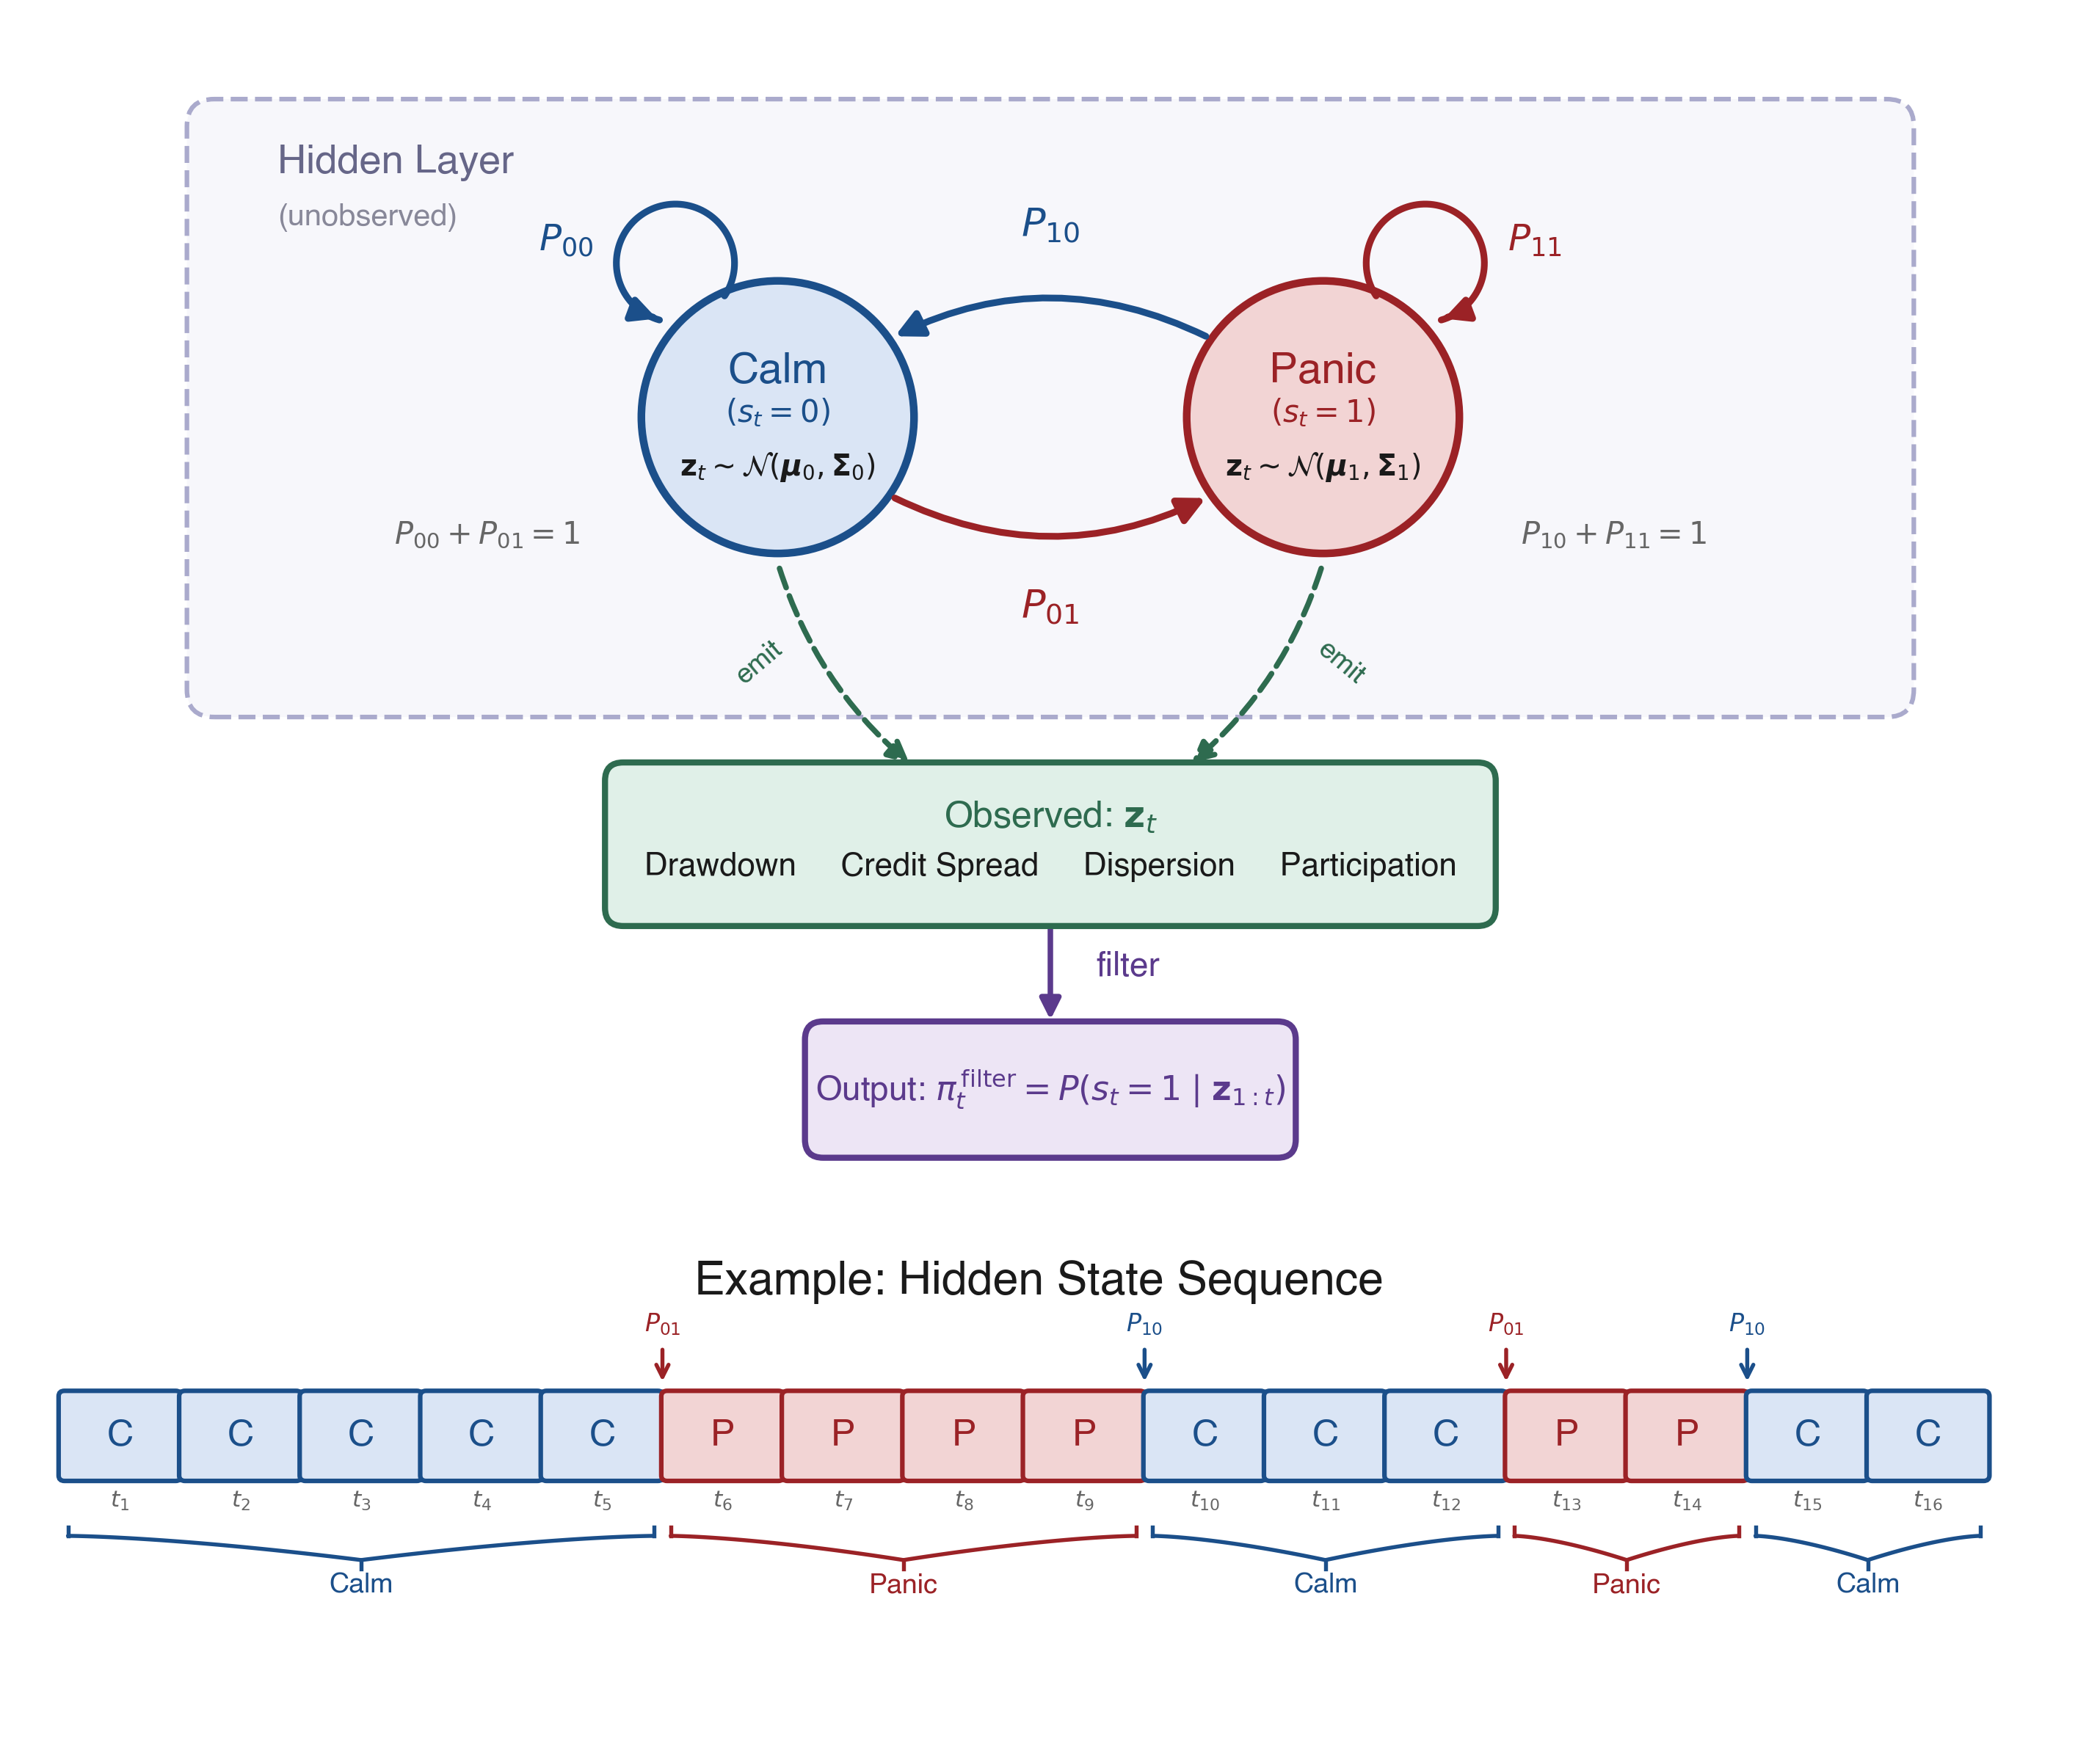
\includegraphics[width=\textwidth]{plots/thesis/markov_chain_diagram.png}
    \caption{Architecture of the two-state Hidden Markov Model. Hidden states (Calm/Panic) evolve via transition probabilities $P_{ij}$ and emit the four-dimensional observation vector $\mathbf{z}_t$. The forward filter inverts this process to produce $\pi_t^{\text{filter}} = P(s_t = 1 \mid \mathbf{z}_{1:t})$. The lower panel shows an example state sequence illustrating regime persistence and abrupt transitions.}
    \label{fig:hmm_diagram}
\end{figure}

\subsubsection{Bayesian Estimation via Gibbs Sampling}\label{sec:gibbs}

The standard frequentist alternative is the Baum--Welch algorithm \citep{Baum1970}, a special case of Expectation-Maximisation \citep{Dempster1977}, which finds maximum likelihood point estimates.

Maximum likelihood estimation of regime-switching HMMs has several known shortcomings for the present application. The likelihood surface is multimodal, with at minimum two equivalent global optima arising from the invariance of the likelihood under state relabelling, and EM can converge to degenerate solutions in which one regime collapses around a single observation \citep{FruhwirthSchnatter2006}. Both problems are exacerbated for rare regimes: the panic state in this sample contains only 91 monthly observations in training, where the asymptotic standard errors that frequentist inference relies on are unreliable and the information matrix can become near-singular at boundary transition probabilities \citep[footnote 12]{Hamilton1989}. The Bayesian approach addresses these issues directly. Posterior sampling integrates over parameter uncertainty rather than relying on a point estimate; conjugate priors regularise rare-regime estimates with explicit, defensible weights (Section~\ref{sec:priors}); and convergence diagnostics across multiple chains (Section~\ref{sec:convergence}) diagnose multimodality that would otherwise go unnoticed under a single EM run.

The Bayesian approach instead draws from the joint posterior:
\[
p\!\left(\{s_t\}_{t=1}^T,\; \{\boldsymbol{\mu}_k,\boldsymbol{\Sigma}_k\}_{k=0}^1,\; \mathbf{P} \,\middle|\, \mathbf{z}_{1:T}\right).
\]
This posterior is not available in closed form because the hidden states and model parameters depend on each other. Therefore we employ Gibbs sampling \citep{AlbertChib1993, Hoff2009}, a Markov chain Monte Carlo (MCMC) method, which resolves this by alternating between three conditional updates: (i) the full hidden state path $\{s_t\}_{t=1}^T$, (ii) the emission parameters $(\boldsymbol{\mu}_k,\boldsymbol{\Sigma}_k)$ for each regime, and (iii) the transition matrix $\mathbf{P}$. Conjugate priors ensure that each block can be sampled exactly from its conditional posterior.

\subsubsection{Prior Specification}\label{sec:priors}

The priors encode two economic beliefs. First, before seeing the data, neither regime should be forced to have extreme values in any feature; the model should learn the characteristics of calm and panic states from the data. Second, regimes should be persistent rather than switching every few months.

\paragraph{Emission parameters}
For each regime $k$, the mean vector and covariance matrix are given a conjugate Normal-Inverse-Wishart (NIW) prior:\footnote{The Inverse-Wishart is a probability distribution over positive-definite matrices, making it the natural prior for a covariance matrix: every sample is guaranteed to be symmetric and positive-definite. The Normal-Inverse-Wishart combines this with a conditional Normal prior on the mean. The prior is called \emph{conjugate} because when the data are Gaussian, the posterior takes the same NIW form with updated hyperparameters, making each Gibbs update an exact draw rather than an approximation.}
\begin{equation}
\boldsymbol{\Sigma}_k \sim \mathcal{IW}(\nu_0,\boldsymbol{\Psi}_0),
\qquad
\boldsymbol{\mu}_k \mid \boldsymbol{\Sigma}_k
\sim
\mathcal{N}\!\left(\mathbf{m}_0,\frac{\boldsymbol{\Sigma}_k}{\kappa_0}\right).
\end{equation}
The hyperparameters are chosen as
\begin{equation}\label{eq:niw_hyperparams}
\mathbf{m}_0 = \mathbf{0},\qquad
\kappa_0 = 0.01,\qquad
\nu_0 = D+2,\qquad
\boldsymbol{\Psi}_0 = \mathbf{I}_D(\nu_0-D-1),
\end{equation}
where $D=4$ is the number of features. After observing data, these prior hyperparameters update to posterior counterparts $\kappa_n$, $\mathbf{m}_n$, $\nu_n$, and $\boldsymbol{\Psi}_n$ (Equation~\ref{eq:niw_update}). Each hyperparameter controls a different aspect of the prior belief:
\begin{itemize}
    \item $\mathbf{m}_0$ is the prior guess for each regime's mean vector. Setting $\mathbf{m}_0 = \mathbf{0}$ reflects that, since all features are standardized, there is no reason to expect either regime to be centered away from zero before seeing the data.
    \item $\kappa_0$ controls how strongly the prior mean $\mathbf{m}_0$ is trusted relative to the data. The very small value $\kappa_0 = 0.01$ makes this prior nearly uninformative, so the posterior mean is driven overwhelmingly by the observed data.
    \item $\nu_0$ is the degrees of freedom of the Inverse-Wishart prior, interpretable as the number of pseudo-observations the prior is worth. The value $\nu_0 = D + 2 = 6$ is the smallest integer for which the prior expected value exists, yielding the most diffuse valid prior; a larger choice (e.g., $\nu_0 = 9$) would impose stronger confidence that the covariance is close to $\mathbf{I}_D$. With roughly 150 calm and 91 panic months in training, the posterior degrees of freedom ($\nu_n = \nu_0 + n_k$) far exceed the prior, so the data dominate the covariance estimates.
    \item $\boldsymbol{\Psi}_0$ is the scale matrix of the Inverse-Wishart prior. It is calibrated so that the prior expected covariance equals the identity matrix, $\mathbb{E}[\boldsymbol{\Sigma}_k] = \boldsymbol{\Psi}_0 / (\nu_0 - D - 1) = \mathbf{I}_D$, implying unit marginal variance and no cross-feature correlation before observing the data.
\end{itemize}

\paragraph{Transition matrix}
Each row of the transition matrix is assigned an independent Dirichlet prior:
\begin{equation}
\mathbf{P}_{0,\cdot} \sim \text{Dir}(9,1),
\qquad
\mathbf{P}_{1,\cdot} \sim \text{Dir}(1,9).
\label{eq:dirichlet_prior}
\end{equation}
Equivalently, in matrix form,
\[
\boldsymbol{\alpha}_{\text{dir}}
=
\left(\begin{array}{cc}
9 & 1 \\
1 & 9
\end{array}\right).
\]
This prior favors persistence in both regimes: absent data, the prior mean transition matrix is
\begin{equation}
\mathbb{E}[\mathbf{P}] =
\left(\begin{array}{cc}
0.90 & 0.10 \\
0.10 & 0.90
\end{array}\right).
\label{eq:prior_mean_P}
\end{equation}
In other words, the prior expects each regime to continue with probability $0.9$, corresponding to an expected duration of roughly $10$ months. This prior is informative enough to discourage pathological solutions but weak enough to be overridden by the data.

\subsubsection{Gibbs Sampling Algorithm}\label{sec:gibbs_sampler}

\paragraph{Initialization}
The Gibbs sampler requires starting values for the emission parameters and the transition matrix. A crude drawdown-based partition is used:\footnote{The choice of initialization has negligible impact on the posterior: the sampler is run for 2{,}000 iterations with 500 discarded as burn-in, and convergence diagnostics (Section~\ref{sec:convergence}) confirm that the chain mixes well regardless of the starting partition.} months with below-median drawdown $DD_t^z$ (i.e., deeper drawdowns) are initially assigned to the panic state ($s_t=1$), and the remaining months to the calm state ($s_t=0$). The initial emission parameters are then computed from each group:
\[
\boldsymbol{\mu}_k^{(0)} = \frac{1}{n_k}\sum_{t:\,s_t=k}\mathbf{z}_t,
\qquad
\boldsymbol{\Sigma}_k^{(0)} = \text{Cov}(\{\mathbf{z}_t : s_t=k\}),
\]
where $n_k$ is the number of months assigned to regime $k$. The initial transition matrix is set to the prior mean, $\mathbf{P}^{(0)} = \mathbb{E}[\mathbf{P}]$ (Equation~\ref{eq:prior_mean_P}). These initial parameters give the first forward pass (described below) emission densities that can distinguish the two states.

\paragraph{Iterative updates}
Each iteration cycles through the three conditional updates described in Section~\ref{sec:gibbs}. Figure~\ref{fig:gibbs_diagram} summarizes the cycle graphically.

\begin{figure}[H]
    \centering
    \vspace{-0.5cm}
    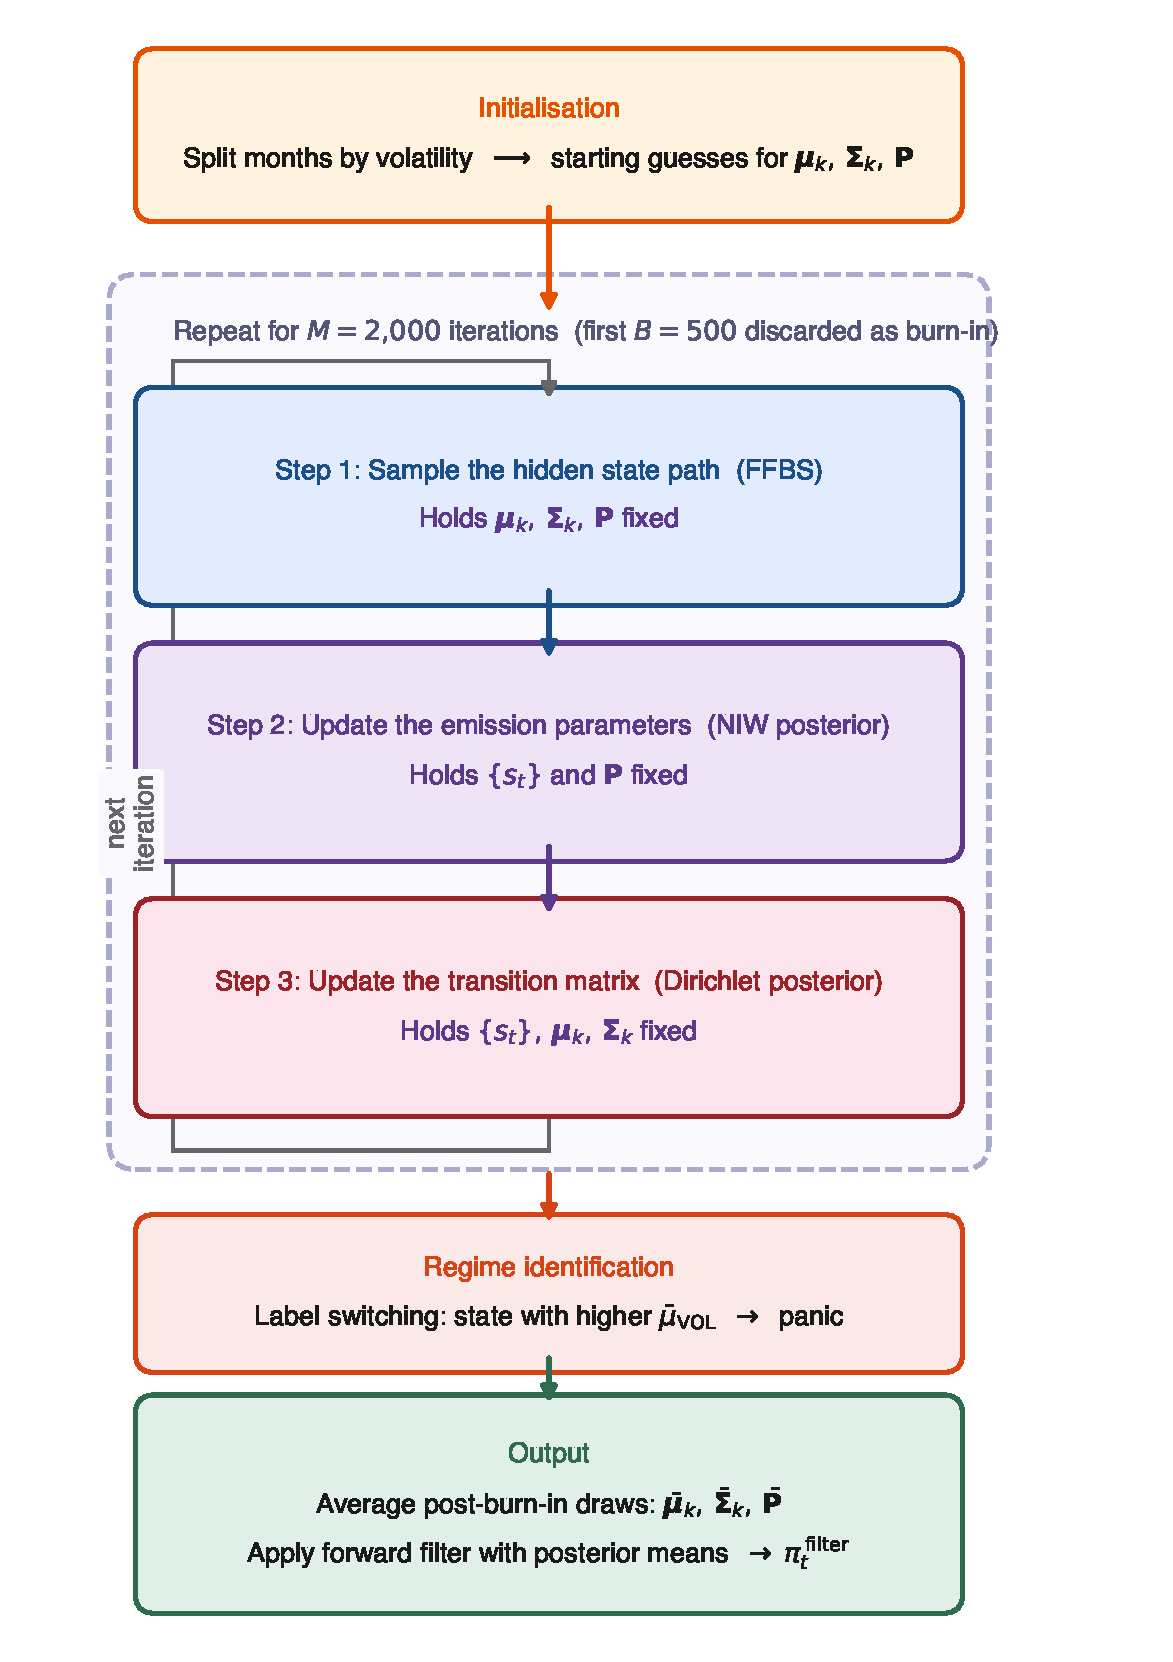
\includegraphics[width=0.88\textwidth]{plots/thesis/gibbs_sampling_diagram.pdf}
    \vspace{-0.3cm}
    \caption{Flowchart of the Gibbs sampler. The dashed loop repeats for $M = 2{,}000$ iterations ($B = 500$ burn-in). Each box shows the conditional posterior being sampled and which parameters are held fixed.}
    \label{fig:gibbs_diagram}
\end{figure}

\paragraph{Step 1: Sampling the hidden state path via FFBS}

The full latent regime sequence $(s_1,\dots,s_T)$ is sampled using Forward-Filtering Backward-Sampling \citep[FFBS; see][ch.~11]{FruhwirthSchnatter2006}, holding the current emission parameters and transition matrix fixed.

The forward pass computes the filtered probability $\alpha_t(k) = P(s_t=k \mid \mathbf{z}_{1:t})$, the probability of being in state $k$ at time $t$ given all observations so far. This quantity is built in two sub-steps. First, a \emph{prediction step} asks: before seeing this month's data, how likely is each state? Since the previous state is unknown, the algorithm sums over both possibilities, weighting each by its filtered probability from the previous month and the transition probability:
\[
\alpha_{t|t-1}(k) = \alpha_{t-1}(0)\,P_{0k} + \alpha_{t-1}(1)\,P_{1k}.
\]
Second, an \emph{update step} revises this prediction once the current observation $\mathbf{z}_t$ arrives, using Bayes' rule: if the observed features look more like a panic month than a calm month, the probability of panic increases. Combining the two steps yields the recursion
\begin{equation}
\alpha_t(k)
=
\frac{f(\mathbf{z}_t \mid s_t=k)\;\alpha_{t|t-1}(k)}
     {f(\mathbf{z}_t \mid s_t=0)\;\alpha_{t|t-1}(0) + f(\mathbf{z}_t \mid s_t=1)\;\alpha_{t|t-1}(1)},
\label{eq:forward_plain}
\end{equation}
where $f(\mathbf{z}_t \mid s_t=k) = \mathcal{N}(\mathbf{z}_t;\boldsymbol{\mu}_k,\boldsymbol{\Sigma}_k)$ is the Gaussian emission density.\footnote{In practice, these densities can be extremely small (or large) for four-dimensional observations, leading to numerical underflow. The implementation avoids this by working in log-space: log-likelihoods $\log f(\mathbf{z}_t \mid s_t = k)$ are computed directly, and the log-sum-exp identity $\log(e^a + e^b) = \max(a,b) + \log(1 + e^{-|a-b|})$ is used whenever probabilities must be normalised.} The recursion is initialized with $\alpha_0(k) = 1/2$, reflecting no prior preference for either regime.

The forward pass tells us how likely each regime is at every month, but if we simply flipped a weighted coin independently at each $t$ we could produce implausible paths (for example, rapid calm-panic-calm-panic switching even though the transition matrix says regimes persist for roughly ten months). The backward pass prevents this by sampling states in reverse: once a future state has been drawn, the current state is sampled conditional on it, so the entire path respects the Markov transition dynamics.

The backward pass proceeds in two steps:

\paragraph{Terminal state} At $t = T$, the filtered probability already conditions on all observations, so the terminal state is drawn directly:
\[
s_T \sim \text{Cat}(\alpha_T(0),\, \alpha_T(1)),
\]
that is, the algorithm draws $s_T = 0$ (calm) with probability $\alpha_T(0)$ and $s_T = 1$ (panic) with probability $\alpha_T(1)$.\footnote{$\text{Cat}$ denotes the categorical distribution, the standard notation for a single draw from a discrete probability vector. With two states it reduces to a weighted coin flip.}

\paragraph{Backward recursion} For each earlier time step $t = T-1, T-2, \dots, 1$, the algorithm chooses a state consistent with two pieces of information: (i) the filtered belief $\alpha_t(k)$ from the forward pass, and (ii) the already-sampled future state $s_{t+1}$, which constrains the current state via the transition probability $P_{k, s_{t+1}}$. Combining these two terms and normalising gives:
\begin{equation}
P(s_t = k \mid s_{t+1}, \mathbf{z}_{1:t}) = \frac{\alpha_t(k)\,P_{k,s_{t+1}}}
{\alpha_t(0)\,P_{0,s_{t+1}} + \alpha_t(1)\,P_{1,s_{t+1}}}.
\label{eq:backward_sampling}
\end{equation}
For example, if the forward filter assigns high probability to calm at time $t$ ($\alpha_t(0)$ is large) and the already-sampled $s_{t+1}$ is also calm (so $P_{0,0}$ is large), then the numerator for $k=0$ dominates and the algorithm will very likely sample $s_t = 0$.

The output of the full FFBS procedure is one draw from the posterior over state paths. Across Gibbs iterations, different paths are sampled, exploring the full posterior uncertainty.

Importantly, the backward pass is used only during training to improve posterior parameter estimates. The trading signal $\pi_t^{\text{filter}}$ relies solely on the causal forward filter.

\paragraph{Step 2: Updating the emission parameters}

Given the sampled state path, each regime $k$ has $n_k$ observations assigned to it. From these, two summary statistics are computed: the sample mean $\bar{\mathbf{x}}_k = \frac{1}{n_k}\sum_{t:\,s_t=k}\mathbf{z}_t$ and the scatter matrix $\mathbf{S}_k = \sum_{t:\,s_t=k}(\mathbf{z}_t - \bar{\mathbf{x}}_k)(\mathbf{z}_t - \bar{\mathbf{x}}_k)^\top$. The posterior hyperparameters are:
\begin{align}\label{eq:niw_update}
\kappa_n &= \kappa_0 + n_k, \qquad
\mathbf{m}_n = \frac{\kappa_0 \mathbf{m}_0 + n_k \bar{\mathbf{x}}_k}{\kappa_n}, \qquad
\nu_n = \nu_0 + n_k, \notag \\[6pt]
\boldsymbol{\Psi}_n &= \boldsymbol{\Psi}_0 + \mathbf{S}_k + \frac{\kappa_0 n_k}{\kappa_n}(\bar{\mathbf{x}}_k-\mathbf{m}_0)(\bar{\mathbf{x}}_k-\mathbf{m}_0)^\top.
\end{align}
Since $\kappa_0 = 0.01 \ll n_k$, the posterior is driven almost entirely by the data.

New regime parameters are then drawn from the updated posterior:
$\boldsymbol{\Sigma}_k \sim \mathcal{IW}(\nu_n,\boldsymbol{\Psi}_n)$ and
$\boldsymbol{\mu}_k \mid \boldsymbol{\Sigma}_k \sim \mathcal{N}(\mathbf{m}_n, \boldsymbol{\Sigma}_k / \kappa_n)$.

\paragraph{Step 3: Updating the transition matrix}

The sampled path is scanned to count transitions: $n_{ij} = \sum_{t=2}^T \mathds{1}(s_{t-1}=i,\, s_t=j)$ records how many times the path moved from state $i$ to state $j$. For example, if the sampled path contains 140 calm-to-calm transitions and 10 calm-to-panic transitions, then $n_{00} = 140$ and $n_{01} = 10$. These observed counts are added to the Dirichlet prior pseudo-counts to obtain the posterior:
\begin{equation}
\mathbf{P}_{i,\cdot} \mid \{s_t\}
\sim
\text{Dir}\!\big(\alpha_{i0} + n_{i0},\; \alpha_{i1} + n_{i1}\big).
\label{eq:dirichlet_update}
\end{equation}
For row 0 (calm), the prior pseudo-counts are $(\alpha_{00}, \alpha_{01}) = (9, 1)$ from Equation~\eqref{eq:dirichlet_prior}, so the posterior becomes $\text{Dir}(9 + 140,\; 1 + 10) = \text{Dir}(149,\; 11)$. The expected persistence probability under this posterior is $149/160 = 0.93$, reflecting that the data reinforced the prior belief in regime persistence. A new transition matrix row is then drawn from this Dirichlet distribution, and the same procedure is applied independently to row 1 (panic).

With all three blocks updated, the sampler returns to Step~1. After sufficient iterations the draws converge to samples from the joint posterior.

\subsubsection{Implementation and Convergence}\label{sec:implementation}

The Gibbs sampler is estimated on the training sample only. To reduce sensitivity to MCMC initialization, the full sampler is run independently with $N_s = 200$ different random seeds. Each chain is run for $M=2{,}000$ iterations with the initialization described above. The first $B=500$ iterations are discarded as burn-in, leaving $1{,}500$ posterior draws per seed.

For each seed, posterior mean parameters $\bar{\boldsymbol{\mu}}_k$, $\bar{\boldsymbol{\Sigma}}_k$, and $\bar{\mathbf{P}}$ are computed by averaging over the post-burn-in draws. A causal forward filter is then applied to the full sample using these parameters to obtain a seed-specific filtered probability $\pi_t^{\text{filter},(s)}$. The final trading signal is the average across seeds:
\begin{equation}
\pi_t^{\text{filter}} = \frac{1}{N_s} \sum_{s=1}^{N_s} \pi_t^{\text{filter},(s)}.
\end{equation}
This Bayesian model averaging is a methodological requirement, not a performance optimisation: with a single Gibbs chain the out-of-sample Sharpe has mean 1.04 and interquartile range 0.10 across random HMM seed draws, while averaging 50 chains raises the mean to 1.09 and collapses the IQR to 0.02 (Appendix~\ref{app:seed_convergence}). The 1.11 figure reported in Section~\ref{sec:results} therefore reflects the production 200-seed configuration and should be interpreted as a posterior-averaged quantity rather than a single-chain point estimate.

\paragraph{Convergence Diagnostics}\label{sec:convergence}

Convergence is assessed in two ways. First, trace plots of the regime means and persistence probabilities are visually inspected to verify that the chain mixes around a stable posterior region after burn-in. Second, effective sample sizes (ESS) are computed for key parameters. Because successive MCMC draws are autocorrelated, $n$ draws from the chain contain less information than $n$ independent samples. The ESS quantifies the number of truly independent draws the chain is equivalent to. For a post-burn-in chain of length $n$,
\begin{equation}
ESS
=
\frac{n}{1 + 2\sum_{\ell=1}^{L^\ast}\hat{\rho}(\ell)},
\end{equation}
where $\hat{\rho}(\ell)$ is the estimated autocorrelation at lag $\ell$,\footnote{$\hat{\rho}(\ell) = \frac{1}{(n-\ell)\,\hat{\sigma}^2}\sum_{i=1}^{n-\ell}(\theta_i - \bar{\theta})(\theta_{i+\ell} - \bar{\theta})$, where $\theta_i$ is the $i$-th post-burn-in draw, $\bar{\theta}$ its sample mean, and $\hat{\sigma}^2$ its sample variance.} and $L^\ast$ is the first lag at which the autocorrelation becomes negative. High ESS indicates that the chain provides many effectively independent posterior draws.\footnote{An ESS of at least 100 per parameter is a common minimum for reliable posterior inference \citep{Gelman2013}.}

While ESS measures efficiency within a single chain, it cannot detect whether different chains have converged to different modes. The Gelman--Rubin $\hat{R}$ statistic \citep{Gelman2013} addresses this by comparing within-chain and between-chain variance across $M$ independent chains, each of length $n$. Let $s_m^2$ denote the variance of chain $m$ and $\bar{\theta}_m$ its mean. The within-chain variance is:
\begin{equation}
    W = \frac{1}{M} \sum_{m=1}^{M} s_m^2,
\end{equation}
and the between-chain variance is:
\begin{equation}
    B = \frac{n}{M-1} \sum_{m=1}^{M} (\bar{\theta}_m - \bar{\theta})^2,
\end{equation}
where $\bar{\theta} = \frac{1}{M}\sum_m \bar{\theta}_m$. If all chains have converged to the same posterior, $B$ should be small relative to $W$. The diagnostic is:
\begin{equation}
    \hat{R} = \sqrt{\frac{\hat{V}}{W}}, \qquad \hat{V} = \frac{n-1}{n}\,W + \frac{B}{n}.
\end{equation}
Values of $\hat{R}$ near 1.0 indicate convergence; the standard threshold is $\hat{R} < 1.1$. To evaluate convergence, five of the 200 chains are selected at random. For the selected feature set (DD+DISP+REL\_N+CS), all parameters have $\hat{R} < 1.01$ (Appendix~\ref{app:gelman_rubin}).

Trace plots of the regime means and persistence probabilities (Figure~\ref{fig:convergence_trace}, Appendix~\ref{app:convergence}) provide visual confirmation that all chains converge to stable posterior values after the burn-in period.

\subsubsection{Regime Identification and Trading Signal}\label{sec:regime_signal}

\paragraph{Label Switching and Regime Naming}\label{sec:label_switching}

In a two-state HMM, the labels $0$ and $1$ are intrinsically arbitrary: relabeling the states leaves the likelihood unchanged. To identify which state corresponds to panic, the known crisis-period behavior of each feature is used.\footnote{The sign directions are determined by a data-driven procedure comparing crisis and non-crisis 95th percentiles; see Appendix~\ref{app:label_switching} for details.} Two features rise during crises (DISP: $+1$, CS: $+1$) and two fall (DD: $-1$, REL\_N: $-1$). The regime whose posterior mean best aligns with these crisis directions is designated as ``panic''; if the Gibbs sampler assigns the panic characteristics to state~0 rather than state~1, the labels are swapped so that $\pi_t^{\text{filter}}$ always represents the probability of the panic state.

Two caveats follow from this naming convention. The HMM identifies two regimes by clustering on the emission features; the label ``panic'' is then assigned to the cluster whose posterior mean aligns with crisis directions. The label therefore reflects a statistical resemblance to historical crisis periods rather than a directly observed market state. Relatedly, the economic interpretations used later in the thesis (liquidity pressure, constrained arbitrage) are readings of what this cluster \emph{likely} corresponds to given the features it loads on, not direct identification claims about the underlying mechanism.

\paragraph{Filtered Regime Probability}\label{sec:trading_signal}

Using the posterior mean parameters $\bar{\boldsymbol{\mu}}_k$, $\bar{\boldsymbol{\Sigma}}_k$, and $\bar{\mathbf{P}}$ from Section~\ref{sec:implementation}, the forward recursion (Equation~\ref{eq:forward_plain}) is applied to the full sample to obtain:
\begin{equation}
\pi_t^{\text{filter}}
=
P(s_t=\text{panic} \mid \mathbf{z}_{1:t};\,\bar{\boldsymbol{\mu}},\bar{\boldsymbol{\Sigma}},\bar{\mathbf{P}}).
\end{equation}
A value near $0$ indicates high confidence in calm, near $1$ indicates panic, and intermediate values reflect genuine ambiguity. This filtered probability serves as the regime signal passed to the portfolio construction methods in Section~\ref{sec:methods}. Figure~\ref{fig:regime_probabilities} and Table~\ref{tab:hmm_separation} in Section~\ref{sec:data} visualise the resulting signal and confirm that the two regimes are meaningfully distinct.

\subsection{Stage 2: Regime-Conditioned Portfolio Construction}\label{sec:stage2}

The filtered regime probability $\pi_t^{\text{filter}}$ from Stage~1 provides a monthly measure of market stress, but on its own it does not select stocks. This stage translates the regime signal into cross-sectional portfolios. Three cross-sectional stock selection methods of increasing complexity are developed: a deterministic regime-adaptive momentum formula (DET), a logistic regression classifier (LR), and an XGBoost gradient-boosted tree regressor (XGB). Each method combines $\pi_t^{\text{filter}}$ with momentum signals at multiple horizons to produce a monthly score for every stock, which is then used to rank stocks into a long-short portfolio: the top decile (using NYSE breakpoints) forms the long leg, the bottom decile forms the short leg, and both legs are value-weighted. The stock-level inputs (momentum horizons and the regime signal) are described in Section~\ref{sec:data}.

A key distinction from standard momentum strategies is worth emphasising. In the traditional approach \citep{JegadeeshTitman1993}, stocks are ranked directly by their raw trailing return at a fixed lookback, so the long leg always holds the stocks with the \emph{highest} momentum and the short leg holds the \emph{lowest}. Here, by contrast, stocks are ranked by their predicted forward return, a learned function of multiple momentum horizons and the regime signal. Because the model learns which momentum \emph{level} is associated with future outperformance in a given market state, the long leg need not contain high-momentum stocks at all: in deep crisis, the model may assign the highest predicted returns to stocks whose momentum is below the cross-sectional average at every horizon (Section~\ref{sec:heterogeneity_picks}). The portfolio construction remains identical (top and bottom deciles), but the criterion for entering each decile is regime-dependent rather than fixed.

The deterministic formula serves as a transparent baseline that tests whether simply varying the momentum lookback horizon with market conditions adds value. The two machine learning methods go further by jointly learning how momentum at multiple horizons and the regime signal interact to predict forward returns. We evaluate every method in long-short construction rather than long-only, for three reasons. First, a long-short portfolio nets out market beta on the two sides, so the remaining return reflects the cross-sectional ranking itself rather than a levered market bet. Second, the regime mechanism this thesis studies is two-sided: in panic the model predicts reversal, meaning it identifies stocks expected to fall as well as stocks expected to rise, and the short leg directly tests whether those downward predictions are informative. Long-only construction would discard that test. Third, long-short is the standard construction in the momentum literature \citep{JegadeeshTitman1993, DanielMoskowitz2016, BarrosoSantaClara2015}, which makes our Sharpe ratios and factor alphas directly comparable to existing results. The results that follow (Section~\ref{sec:results}) not only compare the out-of-sample performance of the three portfolios but also use SHAP values and coefficient analysis to examine \emph{which} features drive the predictions and \emph{how} their importance shifts across calm and panic regimes. This feature-level analysis provides economic insight into the signals that distinguish regime-conditioned stock selection from standard momentum.

\subsubsection{Cross-Sectional Stock Selection Methods}\label{sec:methods}

\paragraph{DET: Deterministic Regime-Adaptive Formula}\label{sec:method0}

The simplest approach exploits the economic intuition that the optimal momentum lookback horizon varies with market conditions. The lookback horizon and stock score are:
\begin{align}
    \ell_t &= \text{clip}\!\left(\text{round}(12 - 11 \cdot \pi_t^{\text{filter}}), \; 1, \; 12\right), \\
    \text{score}_{t}^{\,s} &= \prod_{j=1}^{\ell_t}(1 + r_{t-j}^s) - 1.
\end{align}
Stocks are then ranked by this score; the top decile forms the long leg and the bottom decile the short leg, as described in Appendix~\ref{app:portfolio_construction}.

When $\pi_t^{\text{filter}} \approx 0$ (calm), $\ell_t = 12$, recovering the standard 12-month momentum signal that captures continuation in trending markets \citep{JegadeeshTitman1993}. When $\pi_t^{\text{filter}} \approx 1$ (panic), $\ell_t = 1$, switching to 1-month reversal to exploit the tendency of oversold stocks to recover after panic selling \citep{GHM2023}. At intermediate values, the lookback smoothly interpolates between these extremes.

\paragraph{LR: Logistic Regression}\label{sec:method1}

A logistic regression classifier is trained to predict whether a stock's forward return exceeds the cross-sectional median in each month. Classification is chosen over direct return regression because monthly stock returns are extremely noisy, and predicting the binary outcome ``above or below median'' is a more stable learning target that still produces a useful ranking of stocks. Classification targets have been explored as an alternative to regression in cross-sectional asset pricing, though regression targets generally produce better portfolio performance \citep{Gu2020}; the Ridge regression baseline (Section~\ref{sec:method_ridge}) confirms that the choice of target does not drive the linear model's failure.\footnote{The logistic sigmoid function $\sigma(z) = 1/(1 + e^{-z})$ maps the linear combination $\boldsymbol{\beta}^\top \tilde{\mathbf{x}}$ from the real line to the interval $(0, 1)$, so the output can be interpreted as a probability.}
\begin{equation}
    P(y_t^s = 1 \mid \mathbf{x}_t^s) = \sigma(\boldsymbol{\beta}^\top \tilde{\mathbf{x}}_t^s),
\end{equation}
where $y_t^s = \mathds{1}(r_{t+1}^s > \text{median}_s\{r_{t+1}^s\})$ is a binary label indicating whether stock $s$ outperforms the cross-sectional median in the following month. The feature vector $\tilde{\mathbf{x}}_t^s = (mom_{1,t}^s, \dots, mom_{12,t}^s, \pi_t^{\text{filter}})$ contains the 12 momentum lookbacks and the regime signal, standardized using training-set means and standard deviations. The model is estimated by maximizing the $\ell_2$-regularized log-likelihood:
\begin{equation}
    \hat{\boldsymbol{\beta}} = \arg\max_{\boldsymbol{\beta}} \left[\sum_{i} \Big(y_i \log \sigma(\boldsymbol{\beta}^\top \tilde{\mathbf{x}}_i) + (1 - y_i) \log(1 - \sigma(\boldsymbol{\beta}^\top \tilde{\mathbf{x}}_i))\Big) - \frac{1}{2C} \|\boldsymbol{\beta}\|_2^2\right],
\end{equation}
with regularization strength $C = 1.0$. The $\ell_2$ penalty shrinks coefficients toward zero to guard against overfitting given the large number of correlated momentum features. Once $\hat{\boldsymbol{\beta}}$ is estimated on the training sample, the stock score for any observation is obtained by plugging $\hat{\boldsymbol{\beta}}$ back into the prediction equation:
\begin{equation}
    score_t^s = \sigma(\hat{\boldsymbol{\beta}}^\top \tilde{\mathbf{x}}_t^s) = P(y_t^s = 1 \mid \mathbf{x}_t^s;\, \hat{\boldsymbol{\beta}}).
\end{equation}
Stocks with higher predicted probability of beating the cross-sectional median receive higher scores and are more likely to enter the long leg; those with the lowest scores enter the short leg.

\paragraph{XGB: XGBoost Regressor}\label{sec:method2}

An XGBoost gradient-boosted tree regressor \citep{Chen2016} is trained to predict the forward monthly return directly. Unlike LR, which classifies stocks as above or below the median, XGBoost predicts the forward return directly. This preserves magnitude information: a stock expected to gain 10\% ranks higher than one expected to gain 2\%, a distinction that binary classification discards. The feature vector for each stock-month observation comprises the 13 features described in Section~\ref{sec:cs_features}: the 12 momentum lookbacks ($mom_1, \dots, mom_{12}$) and the regime signal ($\pi_t^{\text{filter}}$). By including all horizons jointly, XGBoost can learn how the full momentum term structure interacts with the regime signal, for example by conditioning its joint use of all 12 horizons on the level of $\pi_t^{\text{filter}}$ in ways that cannot be decomposed into per-horizon slope changes.

XGBoost builds an additive ensemble of $M$ regression trees, where each successive tree fits the residuals of the current ensemble:
\begin{equation}
    F(\mathbf{x}) = \sum_{m=1}^{M} \eta \cdot h_m(\mathbf{x}),
\end{equation}
where $h_m$ is the $m$-th decision tree and $\eta$ is the learning rate that shrinks each tree's contribution to prevent overfitting. Each tree $h_m$ is grown to minimize a regularized objective combining the squared-error loss on the current residuals with penalty terms on tree complexity (number of leaves and leaf weights). The predicted return $\hat{r}_{t+1}^s = F(\mathbf{x}_t^s)$ serves as the stock score. The model is trained with $M = 500$ trees, a learning rate of $\eta = 0.05$, maximum tree depth of 4, and row and column subsampling rates of 0.8. To reduce sensitivity to random initialization, an ensemble of 50 independent XGBoost models (each with a different random seed) is trained; their predictions are averaged before ranking stocks into portfolio deciles.

A maximum depth of 4 allows the model to capture up to four-way feature interactions. The choice of depth is consequential: depth~1 permits no interactions between features, depth~2 permits only pairwise interactions (e.g., one split on $\pi_t^{\text{filter}}$ followed by one split on a single momentum horizon), and depth~$\geq 3$ permits higher-order conditioning across multiple horizons simultaneously. The depth was selected via cross-validation on the 1990--2010 training sample (Appendix~\ref{app:xgb_sensitivity}); Table~\ref{tab:xgb_hyperparams} reports the corresponding out-of-sample sweep as a diagnostic, not as the selection criterion. Annualised return rises monotonically from depth~1 ($8.7\%$, Sharpe $0.53$) through depth~4 ($21.7\%$, Sharpe $1.11$), with the largest gains at depths~2 and~3 where the model first gains multi-way conditioning. A depth-2 model, which conditions on $\pi_t^{\text{filter}}$ and one momentum horizon per tree, achieves $15.7\%$, $28\%$ below the full model. Volatility is nearly constant across depths ($\approx 19.5\%$): deeper trees improve signal quality rather than amplifying risk-taking. The $K=4$ cluster decomposition in Section~\ref{sec:heterogeneity_picks} provides a specific account of why depth~4 is exactly the right budget: distinguishing the four multi-horizon shapes within a $\pi_t^{\text{filter}}$-conditional tree branch requires depth~1 for the regime gate plus at least depth~3 for within-regime shape reading. Performance peaks at depth~4 and declines beyond depth~5.\label{sec:depth_analysis}

The value of the regime signal is architecture-dependent: a depth-matched Random Forest on the same 13 features achieves only Sharpe $0.73$ and demotes $\pi_t^{\text{filter}}$ to $18\%$ of total SHAP (versus $45\%$ for XGBoost; Appendix~\ref{app:xgb_sensitivity}). XGBoost is chosen because its sequential residual fitting concentrates splits on whichever feature most reduces error, turning the regime signal into the model's primary gating variable rather than one feature among thirteen.

\paragraph{Isolating Linearity from the Training Target}\label{sec:method_ridge}

LR and XGB differ not only in functional form (linear vs.\ nonlinear) but also in their training targets: LR predicts a binary classification label, while XGB predicts the continuous forward return. To ensure that any performance difference reflects linearity rather than the choice of target, a Ridge regression baseline is included. Ridge regression is a linear model (identical functional form to logistic regression) that predicts continuous forward returns (identical target to XGBoost), using the same 13 standardised features:
\begin{equation}
    \hat{r}_{t+1}^s = \boldsymbol{\beta}^\top \tilde{\mathbf{x}}_t^s, \qquad \hat{\boldsymbol{\beta}} = \arg\min_{\boldsymbol{\beta}} \left[\sum_i (r_{i,t+1} - \boldsymbol{\beta}^\top \tilde{\mathbf{x}}_i)^2 + \alpha \|\boldsymbol{\beta}\|_2^2\right],
\end{equation}
with $\alpha = 1.0$. Results are robust across regularisation strengths from $\alpha = 0.01$ to $\alpha = 1{,}000$ (Appendix~\ref{app:ridge}). If Ridge regression succeeds where logistic regression fails, the classification target is the bottleneck; if both linear models fail, linearity itself is the constraint.

\paragraph{The Role of $\pi_t^{\text{filter}}$}\label{sec:pi_context}

A key distinction between the linear models (LR and Ridge) and XGB lies in how each model uses the regime signal. A linear model assigns $\pi_t^{\text{filter}}$ a single coefficient, which is near zero because the regime signal is not a direct return predictor. XGBoost, by contrast, uses $\pi_t^{\text{filter}}$ as a context variable through tree splits, conditioning its joint use of all momentum horizons on the current market state. This conditioning operates through multi-dimensional feature interactions \citep{Gu2020} and cannot be represented by a single linear coefficient or decomposed into per-feature slope changes. The empirical consequences of this distinction are analysed in Section~\ref{sec:regime_results}.

With the two-stage framework in place, the next section describes the data, sample construction, and the feature selection procedure used to choose the HMM's input features.
